\section{Yocto: pour qui ? pourquoi?}

Pour construire son OS aujourd'hui, il existe de nombreux outils. Un outils (ou plutôt ensemble d'outils) très utilisé est buildroot. Mais il en exeiste plein d'autre.
Dans le monde de l'industrie le projet Yocto est de plus en plus présent et nous allons voir pourquoi.
\subsection{Les outils disponibles pour construire son OS aujourd'hui}
\paragraph{}

Comme nous l'avons dit, les outils permettant la création d'OS sont multiples.
Voici une synthèse des principaux :
\paragraph{}
Do It Yourself : limité aux cas simples
\begin{itemize} 

\item Avantage = maîtrise totale

\item Inconvénient = il faut tout faire
\end{itemize} 

\paragraph{}
Buildroot : simple mais fonctionnellement moins
riches que les autres
\begin{itemize} 

\item Adapté aux applications enfouies, pas très riches

\item Difficile de travailler en différentiel : régénération complète du
File System, pas de gestion de paquets

\item Basé sur des Makefiles
\end{itemize} 

\paragraph{}
Scratchbox : riche mais obsolète

\paragraph{}
LTIB : outil utilisé par Freescale, mais changement en
cours au profit du Yocto Project

\begin{itemize} 

\item Versions logicielles datées (host + target)

\end{itemize} 



\paragraph{}
OpenEmbedded : Ancêtre commun issu du projet Open Zaurus, toujours actif.
\begin{itemize} 

\item Base de distributions variées

\end{itemize} 
\paragraph{}
Et il en existe encore bien d'autre. Mais alors avec cette forte diversité pourquoi choisir YOCTO ?
Les avantages sont multiples bien sûr, mais le plus important est son côté modulable.
Aussi, ce projet permet de mettre en place de manière industrielle des outils de création de distribution Linux embarqué. C'est donc un projet oprmisé pour le monde de l'industrie.
En effet, du fait de l'évolution des compasants d'un système il faut avoir une certaine flexibilité sur l'OS que l'on conçoit. Yocto permet cette flexibilité.
De plus, le projet Yocto est sous l'égide de la Linux Foundation ce qui permet une certaine garantie de fonctionnement.
On voit donc un peu plus pourquoi Yocto est apprécié des industriels.
Mais comme nous l'avons vu ce projet ce distingue notamment de par sa fléxibilité.
Nous allons maintenant expliquer comment cette flexibilité est permise.





\subsection{Yocto : un fonctionnement plus flexible}
\begin{figure}[ht!]

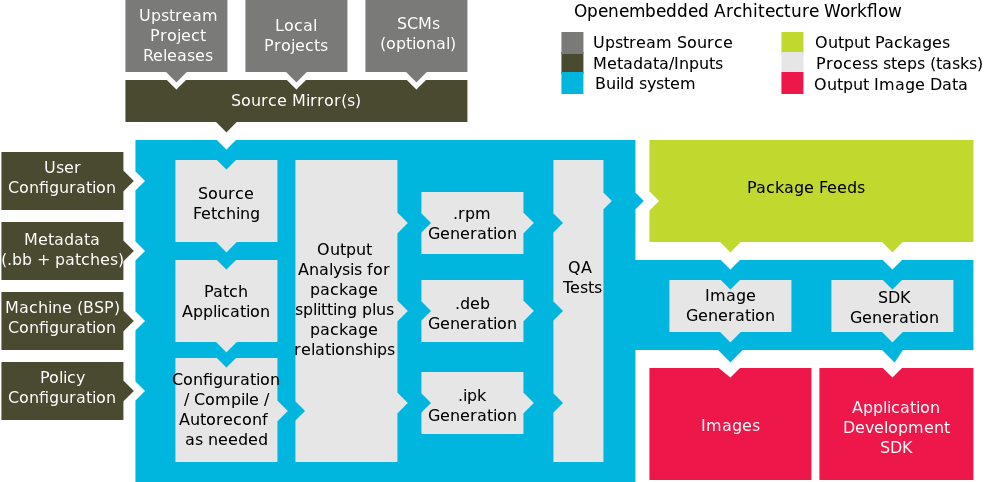
\includegraphics[width=\linewidth]{yocto.png} % Figure image 

\caption{crédit: Yocto project} % Figure caption 


\label{Project Yocto} % Label for referencing with \ref{bear} 
\end{figure}


\paragraph{}
Yocto intègre des parties développées conjointement pour OpenEmbedded, notamment BitBake, OpenEmbedded-Core et d'autres métadonnées. 
Les éléments développés dans le cadre du projet, appelés "meta-yocto" et "meta-yocto-bsp", comprennent l'intégration des éclipses. 
Ensemble, ils améliorent les outils d'OpenEmbedded, cette plateforme de référence pour la construction de systèmes avancés embarqués dans les HW est connue 
sous le nom de Poky.

Pour développer des logiciels, nous avons besoin d'une chaîne d'outils (croisés) : les fichiers sources et les instructions sur la façon de les compiler. 
C'est suffisant pour une source. 
Pour plus de composants et de dépendances dans la compilation et le temps d'exécution, il faut augmenter la complexité et des étapes supplémentaires. 
Bitbake est un agent ayant la capacité d'interpréter et d'exécuter les recettes d'amélioration, il calcule la chaîne des tâches nécessaires pour développer l'objectif défini et exécuté. 

